\section[Background]{Background \textnormal{\cite{Eichler_2018}}}

Lasers are ubiquitous tools of modern physics due to their useful properties, characterized by the emission of coherent light with narrow
spectral linewidth, low divergence and high power density. They are named after the acronym for light amplification by stimulated emission
of radiation, describing the fundamental mechanism for the production of laser radiation. This will be explored in the following, both in
the general as well as the special case of the \HeNe laser.

\subsection{Components of a laser}

The basic setup of a typical laser consists of three main components, namely an active medium, a pumping mechanism and the resonator cavity.

Inside the active medium, realized using materials such as semiconductors or gas mixtures, photons are emitted from atomic transitions to
energetically lower states. The energy difference $\Delta E$ between the involved electron levels is therefore the main determinant
of wavelength $\lambda$ and frequency $f$ via $\Delta E = hf$.

To excite electrons in the active medium to higher levels, an energy source is required. This is the role of the pumping mechanism, which
can be implemented using electrons or photons. The latter case is called optical pumping, as another separate light source tuned to the
respective $\Delta E$ value is used to induce transitions to excited states.

Amplification of the emitted radiation is achieved in the active medium. Instead of using superradiant lasers, which have high gain factors
and divergence, or impractically long constructions, mirrors can be used to create a resonator cavity. The resulting standing waves correspond
to multiple passes through the material and can generate a stable beam with low divergence, which can exit through a semitransparent window.
The mirror geometry can be adapted to the desired function with flat or concave designs.



\subsection{Processes in the active medium}

There are three main processes shown in Figure \ref{fig:processes} occuring inside the active medium to facilitate the operation of a laser.

\begin{figure}[H]
	\centering
	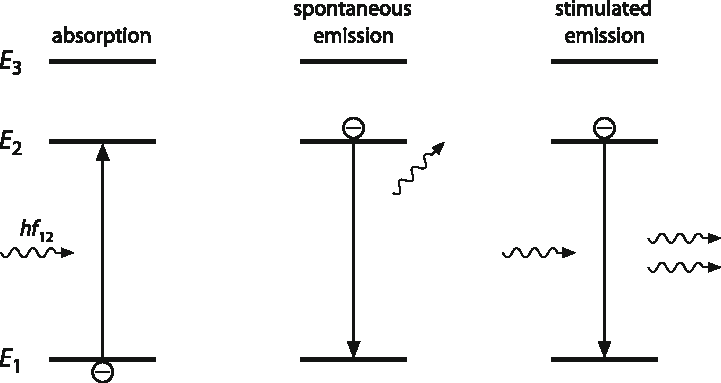
\includegraphics[width=0.65\textwidth]{content/graphics/processes.pdf}
	\caption{Schematic depiction of relevant processes inside the active medium. \cite{Eichler_2018}}
	\label{fig:processes}
\end{figure}

Raising the energy of an electron by $\Delta E = E_2 - E_1$ requires the annihilation of an incident photon that fulfills the condition
\begin{equation*}
	\Delta E = hf_{12} \: ,
\end{equation*}
where $h$ is the Planck constant. This process is referred to as absorption. The number of transitions per time and volume is proportional
to the density of ground state electrons $N_1$ as well as the photon flux or number per area and time $\varphi$ via
\begin{equation*}
	\left. \frac{dN_1}{dt} \right|_\text{ab} = -\sigma_{12} N_1 \varphi \: ,
\end{equation*}
with $\sigma_{12}$ denoting the effective cross section for absorbing a photon. From this also follows the typical exponential intensity
reduction
\begin{equation*}
	\left. \frac{dI}{dx} \right|_\text{ab} = -\sigma_{12} N_1 I \: ,
\end{equation*}
where $\alpha = -\sigma_{12} N_1$ gives the absorption coefficient.

When an atom is in an excited state, it returns to the ground state after a time interval, the duration of which follows some random
distribution with mean lifetime $\tau$. Due to its stochastic nature, this process is called spontaneous emission and has no predefined
direction or phase. The density in the higher level then follows
\begin{equation*}
	\left. \frac{dN_2}{dt} \right|_\text{sp} = - \tau^{-1} N_2 \: .
\end{equation*}

Besides this, emission can also be initiated by an incoming photon of appropriate frequency. This is called stimulated emission and results
in the production of radiation with the same energy, direction and phase as the inducing quantum. As the inverse process to absorption,
\begin{equation*}
	\left. \frac{dN_2}{dt} \right|_\text{st} = -\sigma_{21} N_2 \varphi \: ,
\end{equation*}
describes the time derivative and
\begin{equation*}
	\left. \frac{dI}{dx} \right|_\text{st} = \sigma_{21} N_2 I \: ,
\end{equation*}
the corresponding intensity relation. This means that stimulated emission leads to an increase in intensity, serving as a potential
mechanism for amplification when there are more electrons in the excited state than in the ground state and losses are compensated for.
This phenomenon in referred to as population inversion.

The cross sections can be identified with the Einstein coefficients $B_{ij}$ via
\begin{equation*}
	\sigma_{ij} = B_{ij} h f_{ij} / c \: ,
\end{equation*}
where $c$ is the speed of light in vacuo. Furthermore, for emission and absorption, the thermodynamic or quantum mechanical relation
\begin{equation*}
	\textsl{g}_1 \sigma_{12} = \textsl{g}_2 \sigma_{21}
\end{equation*}
holds, with $\textsl{g}_1$ and $\textsl{g}_2$ defining the degrees of degeneracy for the ground and excited states. Hereafter, it is
assumed that $E_1$ and $E_2$ have the same number of sublevels, so $\textsl{g}_1 = \textsl{g}_2$ for $\sigma_{12} = \sigma_{21}$ and
\begin{equation*}
	B \equiv B_{12} = B_{21} \: .
\end{equation*}
The reciprocal decay timescale defines another Einstein coefficient
\begin{equation*}
	A = \tau^{-1} \: ,
\end{equation*}
with which the stationary spectral radiance
\begin{equation*}
	\rho_s \equiv \pfrac{A}{B \,} = \frac{8\pi h f_{12}^3}{c^3}
\end{equation*}
can be written. Introducing the general spectral radiance
\begin{equation*}
	\rho = \varphi h f_{12} / c
\end{equation*}
and requiring $N = N_1 + N_2$ to be constant for a system of two energy levels, one finds
\begin{equation*}
	\frac{dN_1}{dt} = \left. \frac{dN_1}{dt} \right|_\text{ab} \!\! - \: \left. \frac{dN_2}{dt} \right|_\text{st} \!\! - \:
	\left. \frac{dN_2}{dt} \right|_\text{sp} \!\! = \: \rho B (N_2 - N_1) + AN_2 = - \frac{dN_2}{dt} \: .
\end{equation*}
For $\Delta N = N_2 - N_1$ then follows that
\begin{equation*}
	\pfrac{d\Delta N}{dt} = -2\frac{dN_1}{dt} = -2\rho B \Delta N - 2AN_2 + AN_1 - AN_1 = -2\rho B \Delta N - A\Delta N - AN \: .
\end{equation*}
After some time an equilibrium is reached inside the active medium, resulting in a vanishing time derivative. In this case, solving for the
stationary number difference
\begin{equation*}
	\Delta N_s = -\pfrac{AN}{A + 2\rho B} = -\pfrac{N}{1 + 2\rho / \kern-0.5pt \rho_s}
\end{equation*}
yields $\Delta N_s < 0$ for any system with only two energy levels.



\subsection{Necessity of multiple levels}

This result directly contradicts the requirement of population inversion $\Delta N_s > 0$ necessary for the amplification through stimulated
emission as discussed previously, preventing the usage of two level systems as the active medium. Adding more energy levels as depicted in
Figure \ref{fig:levels} solves this problem. Instead of immediately relaxing back to the ground state via spontaneous emission, excited
electrons now decay very quickly from $E_3$ to $E_2$ and $E_1$ to $E_0$ while the $E_2$ to $E_1$ transition takes longer. This means that
$A_{21} < A_{32}$ as well as $A_{21} < A_{10}$ and results in a distribution similar to what is shown below.

\begin{figure}[H]
	\centering
	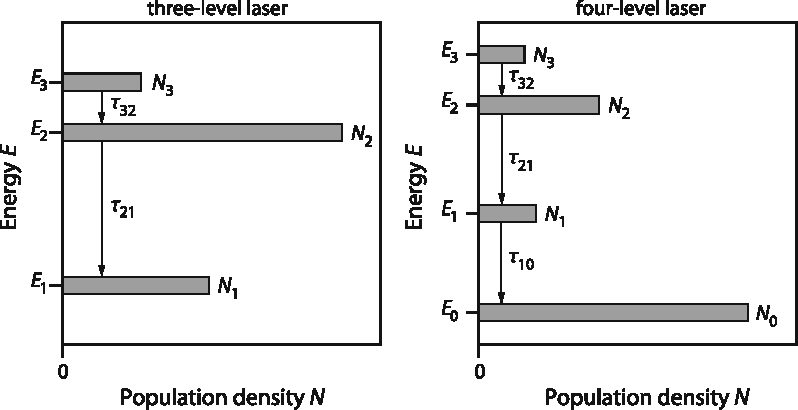
\includegraphics[width=0.70\textwidth]{content/graphics/levels.pdf}
	\caption{Exemplary energies and population densities for multiple levels. \cite{Eichler_2018}}
	\label{fig:levels}
\end{figure}

One then expects $N_0 \kern+0.5pt , N_2 \gg N_1 \kern+0.5pt , N_3$ for $N \approx N_0 + N_2$ and $\Delta N \approx N_2$ in the
stationary configuration. Accordingly, a population inversion $\Delta N_s > 0$ is trivial to achieve, making four level systems a suitable
choice for laser construction.

Such a system is realized by a \HeNe laser 

\begin{figure}[H]
	\centering
	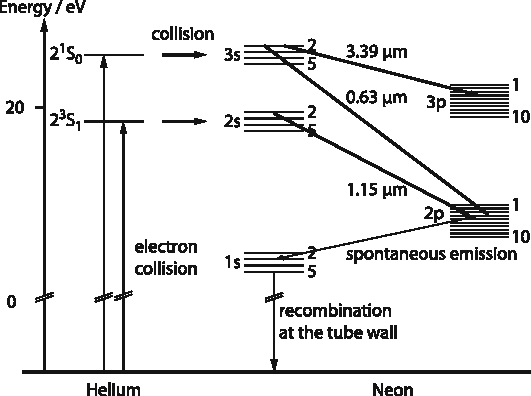
\includegraphics[width=0.60\textwidth]{content/graphics/hene.pdf}
	\caption{Energy level diagram of a \HeNe laser in Paschen notation. \cite{Eichler_2018}}
	\label{fig:hene}
\end{figure}

\begin{table}[H]
	\centering
	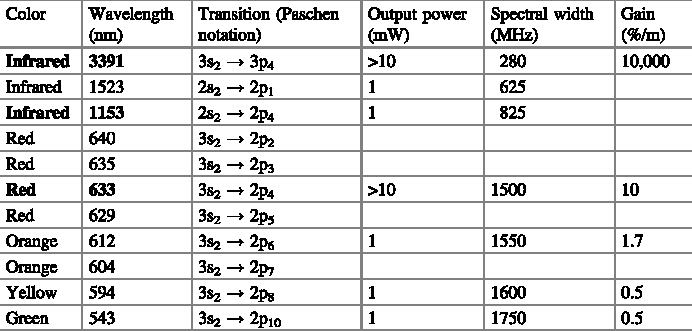
\includegraphics[width=0.80\textwidth]{content/graphics/table.pdf}
	\caption{. \cite{Eichler_2018}}
	\label{fig:table}
\end{table}



\subsection{Stability for different resonators}



\subsection{Transverse and longitudinal modes}



\subsection{Doppler broadening of the transition}



\subsection{Brewster windows and polarization}

\begin{figure}[H]
	\centering
	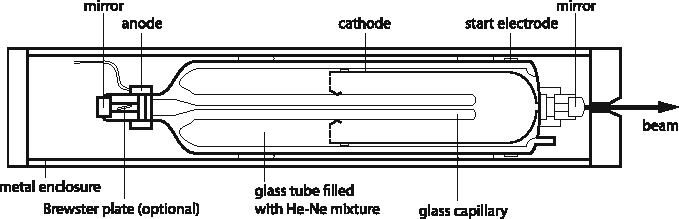
\includegraphics[width=0.60\textwidth]{content/graphics/setup.pdf}
	\caption{. \cite{Eichler_2018}}
	\label{fig:setup}
\end{figure}
